% **************************************************
% Document Class Definition
% **************************************************
\documentclass[%
    paper=A4,               % paper size --> A4 is default in Germany
    twoside=true,           % onesite or twoside printing
    openright,              % doublepage cleaning ends up right side
    parskip=half,           % spacing value / method for paragraphs
    chapterprefix=true,     % prefix for chapter marks
    11pt,                   % font size
    headings=normal,        % size of headings
    bibliography=totoc,     % include bib in toc
    listof=totoc,           % include listof entries in toc
    titlepage=on,           % own page for each title page
    captions=tableabove,    % display table captions above the float env
    chapterprefix=false,    % do not display a prefix for chapters
    appendixprefix=false,    % but display a prefix for appendix chapter
    draft=false,            % value for draft version
]{scrreprt}%


% **************************************************
% Setup YOUR thesis document in this file !
% **************************************************
% !TEX root = my-thesis.tex


% **************************************************
% Files' Character Encoding
% **************************************************
\PassOptionsToPackage{utf8}{inputenc}
\usepackage{inputenc}


% **************************************************
% Information and Commands for Reuse
% **************************************************
\newcommand{\thesisTitle}{Rodamientos Magnéticos Híbridos }
\newcommand{\thesisName}{Bejarano Montiel Omar Alejandro\\ Enriquez Ramirez Oscar\\ Limones Urbina Manuel Enrique}
\newcommand{\thesisSubject}{Informe Técnico}
\newcommand{\thesisDate}{Abril 4, 2016}
\newcommand{\thesisVersion}{Primera}

\newcommand{\thesisFirstReviewer}{M. en C. Alvaro Gordillo Sol}
\newcommand{\thesisFirstSupervisor}{Griselda Sanchez Otero}
\newcommand{\thesisUniversity}{\protect{Instituto Politécnico Nacional}}
\newcommand{\thesisUniversityDepartment}{Unidad Profesional Interdisciplinaria en Ingeniería y Tecnologías Avanzadas}
\newcommand{\thesisUniversityCity}{Ciudad de México}
\newcommand{\thesisUniversityStreetAddress}{Av. Instituto Politécnico Nacional 2580, Gustavo A. Madero, Barrio La Laguna Ticoman}
\newcommand{\thesisUniversityPostalCode}{07340}



% **************************************************
% Debug LaTeX Information
% **************************************************
%\listfiles


% **************************************************
% Load and Configure Packages
% **************************************************
\usepackage[spanish]{babel} % babel system, adjust the language of the content
\PassOptionsToPackage{% setup clean thesis style
    figuresep=colon,%
    hangfigurecaption=false,%
    hangsection=true,%
    hangsubsection=true,%
    colorize=full,%
    colortheme=bluemagenta,%
    bibsys=biber,%
    bibfile=bib-refs,%
    bibstyle=alphabetic,%
}{cleanthesis}
\usepackage{cleanthesis}

%****************
%Other packages
%****************

\hypersetup{% setup the hyperref-package options
    pdftitle={\thesisTitle},    %   - title (PDF meta)
    pdfsubject={\thesisSubject},%   - subject (PDF meta)
    pdfauthor={\thesisName},    %   - author (PDF meta)
    plainpages=false,           %   -
    colorlinks=false,           %   - colorize links?
    pdfborder={0 0 0},          %   -
    breaklinks=true,            %   - allow line break inside links
    bookmarksnumbered=true,     %
    bookmarksopen=true          %
}



% **************************************************
% Document CONTENT
% **************************************************
\begin{document}

% uncomment the following command to fill up pages with
% whitespace instead of aligning the first and last lines
% of a page (see \raggedbottom vs. \flushbottom)
%\raggedbottom

% --------------------------
% rename document parts
% --------------------------
%\renewcaptionname{ngerman}{\figurename}{Abb.}
%\renewcaptionname{ngerman}{\tablename}{Tab.}
\renewcaptionname{english}{\figurename}{Fig.}
\renewcaptionname{english}{\tablename}{Tab.}

% --------------------------
% Front matter
% --------------------------
\pagenumbering{roman}			% roman page numbing (invisible for empty page style)
\pagestyle{empty}				% no header or footers
% !TEX root = ../thesis-example.tex
%
% ------------------------------------  --> cover title page
\begin{titlepage}
	\pdfbookmark[0]{Cover}{Cover}
	\flushright
	\hfill
	\vfill
	{\LARGE\thesisTitle \par}
	\rule[5pt]{\textwidth}{.4pt} \par
	{\Large\thesisName}
	\vfill
	\textit{\large\thesisDate} \\
	Version: \thesisVersion
\end{titlepage}


% ------------------------------------  --> main title page
%\begin{titlepage}
%	\pdfbookmark[0]{Titlepage}{Titlepage}
%	\tgherosfont
%	\centering
%
%	{\Large \thesisUniversity} \\[4mm]
%	%
\includegraphics[width=6cm]{gfx/Clean-Thesis-Logo} \\[2mm]
%	\Large{\thesisUniversityDepartment} \\
%	%\textsf{\thesisUniversityInstitute} \\
%	%\textsf{\thesisUniversityGroup} \\
%
%	\vfill
%	{\large \thesisSubject} \\[5mm]
%	{\LARGE \color{ctcolortitle}\textbf{\thesisTitle} \\[10mm]}
%	{\Large \thesisName} \\
%
%	\vfill
%	\begin{minipage}[t]{.27\textwidth}
%		\raggedleft
%		\textit{Asesor: }
%	\end{minipage}
%	\hspace*{15pt}
%	\begin{minipage}[t]{.65\textwidth}
%		{\Large \thesisFirstReviewer} \\
	  	%{\small \thesisFirstReviewerDepartment} \\[-1mm]

		%{\small \thesisFirstReviewerUniversity}
%	\end{minipage} \\[5mm]
		%\hspace*{15pt}
	%\begin{minipage}[t]{.65\textwidth}
	%	{\Large \thesisSecondReviewer} \\
	%  	{\small \thesisSecondReviewerDepartment} \\[-1mm]
	%	{\small \thesisSecondReviewerUniversity}
	%\end{minipage} \\[10mm]
%	\begin{minipage}[t]{.27\textwidth}
%		\raggedleft
%		\textit{Profesor Titular: }
%	\end{minipage}
%	\hspace*{15pt}
%	\begin{minipage}[t]{.65\textwidth}
%		\thesisFirstSupervisor\ %and \thesisSecondSupervisor
%	\end{minipage} \\[10mm]
%
%	\thesisDate \\
%
%\end{titlepage}

% ------------------------------------  --> lower title back for single page layout
\hfill
\vfill
{
	\small
	\textbf{\thesisName} \\
	\textit{\thesisTitle} \\
	\thesisSubject, \thesisDate \\
	Asesor: \thesisFirstReviewer\\ %and \thesisSecondReviewer \\
	Profesor Titular: \thesisFirstSupervisor\\ %and \thesisSecondSupervisor \\[1.5em]
	\thesisUniversity \\
	%\textit{\thesisUniversityGroup} \\
	%\thesisUniversityInstitute \\
	\thesisUniversityDepartment \\
	\thesisUniversityStreetAddress \\
	\thesisUniversityPostalCode\ , \thesisUniversityCity
}
		% INCLUDE: all titlepages
\cleardoublepage

\pagestyle{plain}				% display just page numbers
% !TEX root = ../my-thesis.tex
%
\pdfbookmark[0]{Abstract}{Abstract}
\addchap*{Abstract}
\label{sec:abstract}

\blindtext

\vspace*{20mm}

{\usekomafont{chapter}Abstract (different language)}
\label{sec:abstract-diff}

\blindtext
		% INCLUDE: the abstracts (english and german)
\cleardoublepage
%


%\pdfbookmark[0]{Acknowledgement}{Acknowledgement}
\chapter*{Nomenclatura}
\label{sec:Acknowledgement}
\vspace*{-10mm}
%\renewcommand{thechapter}{\Roman{Nomenclatura}}
\addcontentsline{toc}{chapter}{Nomenclatura}

\chapter*{Unidades/Simbología}
\label{sec:Acknowledgement}
\vspace*{-10mm}
\addcontentsline{toc}{chapter}{Unidades/Simbología}

\chapter*{Objetivos}
\label{sec:Acknowledgement}
\vspace*{-10mm}
\addcontentsline{toc}{chapter}{Objetivos}

\section*{Objetivo General}
Diseñar y simular un sistema de rodamientos magnéticos capaz de operar en condiciones de carga estática.

\section*{Objetivos Específicos}

{\setlength{\parindent}{0pt}Trabajo Terminal I:}
\begin{enumerate}
\addtolength{\itemsep}{0pt}
\item Obtener el diseño conceptual del rodamiento magnético híbrido.
\item Obtener el diseño conceptual del rodamiento magnético híbrido.
\item Seleccionar el material ferromagnético para el núcleo de los electroimánes. 
\item Calcular la sección transversal de los electroimánes.
\item Obtener la geometría y dimensiones de los rodamientos activos radial y axial.
\item Validar el punto de operación del electroimán mediante simulación.
\item Diseñar un electrodo de alta sensitividad para el rango de operación.
\item Diseñar un dispositivo para la retracción del imán permanente. 
\item Proponer un circuito de adquisición y control. 
\end{enumerate}

Trabajo Terminal II:
\begin{enumerate}
\addtolength{\itemsep}{0pt}
\item Obtener un modelo de electroimánes que integre los efectos del flujo marginal.
\item Realizar las simulaciones de la fuerza magnética ejercida por los electroimánes y el imán permanente.
\item Obtener el modelo dinámico del sistema.  
\item Comparar algunos esquemas de control para la estabilización del sistema.
\item Diseño del circuito de potencia de los electroimánes. 
\item Estimar los límites de operación del rodamiento con base en las simulaciones.
\end{enumerate}
 % INCLUDE: acknowledgement
\cleardoublepage
%
\setcounter{tocdepth}{2}		% define depth of toc
\tableofcontents				% display table of contents
\cleardoublepage

% --------------------------
% Body matter
% --------------------------
\pagenumbering{arabic}			% arabic page numbering
\setcounter{page}{1}			% set page counter
\pagestyle{scrheadings}			% header and footer style

%% Uncomment the following lines using the \part command
%% to add part sections
%\part{Example Part}
% !TEX root = ../thesis-example.tex
%
\chapter{Introducción}			%El [*] para no enumerar el capitulo en la tabla de contenidos
\label{sec:intro}
\addcontentsline{toc}{chapter}{Introducción}	%Para que el capitulo aparezca en la tabla de cont.

\cleanchapterquote{You can’t do better design with a computer, but you can speed up your work enormously.}{Wim Crouwel}{(Graphic designer and typographer)}

El desarrollo de nuevas investigaciones y nuevas tecnologías han permitido que la industria busque nuevas y mejores formas de llevar a cabo sus procesos productivos, lo que requiere, entre otras cosas, de transformar y actualizar la maquinaria y equipo que utilizan con el propósito de volverlos más eficientes y aumentar su productividad.
En este aspecto se han realizado numerosos avances y descubrimientos, como pueden ser el uso de fuentes de energía más limpias y eficientes, la implementación de nuevos materiales más ligeros y resistentes, y por supuesto el reemplazo de algunos componentes y dispositivos por otros más avanzados.
Gran parte de la maquinaria industrial posee elementos de tipo rotativo, los cuales requieren el uso de dispositivos denominados cojinetes, también conocidos como rodamientos o baleros. Estos suelen situarse entre dos componentes de la maquina con un eje de rotación común, facilitando el movimiento de giro de un componente con respecto al otro y reduciendo la fricción de los diferentes elementos móviles; son a su vez, un punto de apoyo para dichos ejes o árboles. 
Además de ser capaces de disminuir la fricción, de manera general los rodamientos deben cumplir con algunas características particulares, como son: disminuir las vibraciones, operar de manera silenciosa y poseer una prolongada vida útil. Sin embargo, los distintos sectores industriales suelen establecer sus propios requisitos específicos con base en determinados entornos operativos o aplicaciones particulares, entre los que podemos mencionar: resistir grandes cambios de temperatura, humedad, suciedad, operar en medios agresivos como soluciones acidas o alcalinas, soportar altas velocidades e incluso ser aptos para el contacto con alimentos \citep{libro_pro}.
Es por ello que dentro de los rodamientos existe una gran variedad de configuraciones, materiales y modos de operación que puedan satisfacer esta demanda de necesidades.


\section*{Clasificación de Cojinetes y Rodamientos}
\label{sec:intro:address}
\addcontentsline{toc}{section}{Clasificación de Cojinetes y Rodamientos}

Los cojinetes se clasifican principalmente en dos grandes grupos: cojinetes de deslizamiento (o de fricción) y antifricción (rodamientos). Los cojinetes de deslizamiento consisten básicamente en un par de casquillos concéntricos que giran en contacto directo uno con el otro realizándose un deslizamiento por fricción, procurando que esta sea la menor posible; la disminución de la fricción depende de los materiales con los que están fabricados y del uso de alguna película lubricante [2]. 
Por su parte, los cojinetes antifricción (rodamientos) comprenden una clasificación más extensa debido a su complejidad estructural, en comparación a los cojinetes de deslizamiento. Entre los principales podemos encontrar: por la dirección de la carga que soportan (axial, radial, angular o mixta, y lineal), según su rigidez (rígidos y pivotantes) y por el tipo de cuerpo rodante (de bolas, rodillos, agujas, cónicos, etc.) [3]. 
El rozamiento por rodadura generado por los rodamientos es mucho menor que el de los cojinetes de deslizamiento, y es por ello que presentan una serie de ventajas más frente a la utilización de casquillos que incluye mayor velocidad admisible, menor temperatura de funcionamiento, mayor capacidad de carga, menor desgaste, facilidad de recambio y disminución en los costos de mantenimiento. 
A pesar de todo esto, existen algunas aplicaciones para las cuales se deben buscar alternativas a estos dispositivos mecánicos, particularmente las que están relacionadas con máquinas rotativas de alta velocidad donde se incrementan de manera considerable las perdidas mecánicas, las cuales están asociadas al rozamiento y a las vibraciones mecánicas. Ante este problema surge un tipo de rodamiento que opera por medio de la suspensión magnética, conocidos como rodamientos magnéticos.  

\section*{Rodamientos Magnéticos}
\label{sec:intro:motivation}
\addcontentsline{toc}{section}{Rodamientos Magnéticos}

Como ya se mencionó anteriormente, los rodamientos magnéticos son una excelente alternativa para su uso en máquinas rotativas de alta velocidad, ya que presentan múltiples ventajas frente a los rodamientos tradicionales, como una mayor velocidad de giro, no requieren de un sistema de lubricación ya que operan sin contacto, por lo que además no producen partículas de desgaste y debido a su baja rigidez son capaces de compensar las vibraciones mecánicas, haciéndolos silenciosos. Todo esto se traduce en una disminución de los costos de mantenimiento y prolongación de la vida útil del sistema. 
El potencial que poseen para generar muy pocas pérdidas y alcanzar mayores velocidades los hace ideales para aplicaciones industriales como centrifugadoras de alta velocidad, volantes inerciales, compresores y turbinas de alto régimen de revoluciones, por mencionar algunas. 
Los rodamientos magnéticos cuentan, a su vez, con una clasificación que viene en función de dos principales factores: de acuerdo a la naturaleza de su fuerza, que puede ser de Reluctancia o de Fuerza de Lorentz, o más comúnmente de acuerdo a la fuente generadora del campo magnético (Pasivos, Activos e Híbridos) [4]. 
Los pasivos carecen de alimentación externa y emplean imanes permanentes para generar los campos magnéticos de levitación, mientras que los activos utilizan electroimanes y requieren de una fuente de alimentación externa y de un sistema de control. Por su parte, los híbridos emplean imanes permanentes para crear un campo base de levitación mientras que el resto del campo es generado por electroimanes.
A pesar de que la mayoría de los usos que se le dan a los rodamientos magnéticos pertenecen al sector aeroespacial, naval, generador de energía y otras aplicaciones de alta demanda, también es posible aprovecharlos en otro tipo de maquinaria más comercial pudiendo explotar al máximo sus beneficios. 


\section*{Antecedentes}
\subsection*{Investigación y Desarrollo de Rodamientos Magnéticos}
\label{sec:intro:results}
\addcontentsline{toc}{section}{Antecedentes}
\addcontentsline{toc}{subsection}{Investigación y Desarrollo de Rodamientos Magnéticos}

Investigación y Desarrollo de Rodamientos Magnéticos 
A pesar de las múltiples ventajas que presentan, los rodamientos magnéticos no están exentos de algunos problemas que pueden dificultar su desarrollo e implementación en los sistemas industriales, entre los que podemos destacar el alto consumo energético que generan.
Ante este problema se hicieron varias investigaciones cuyas soluciones pueden clasificarse en dos tipos: el diseño de algoritmos para minimizar las corrientes en los electroimanes y el uso de imanes permanentes para proveer un campo magnético base para la levitación.
La investigación realizada en [5] se trata de una validación experimental en donde 1) se diseña y construye un prototipo de pruebas que emula el comportamiento de un rodamiento magnético activo de un grado de libertad, y 2) se realizaron pruebas para evaluar el desempeño del controlador inteligente en comparación con un controlador estándar de polarización fija.
Este equipo consiste en un eje rígido capaz de balancearse libremente sobre un punto de apoyo colocado debajo de su centro de masa. La posición angular de este eje es controlada mediante electroimanes fijados a los extremos de este. A pesar su simplicidad este equipo incorpora todas las no linealidades típicas de un rodamiento magnético activo, y la dinámica del sistema es ideal para evaluar el desempeño de los controladores. 
En [6] una estrategia de control de corriente de polarización variable es presentada con el fin de minimizar la energía consumida sin alterar el desempeño dinámico del sistema. El modelado parte de un RMA de 2 polos sobre el cual se propone un controlador lineal y un observador de estados para la estimación de estados.
Una vez obtenido el modelo del sistema se calcula de manera analítica la corriente óptima para la estabilización del sistema y obtener el controlador. 

Como resultado este controlador propuesto fue capaz de reducir el consumo en un 73\%, se estabilizó la posición de rotor en el centro del rodamiento con un error de estado estable nulo y se presentaron vibraciones 60\% menores comparadas con un controlador de polarización fija.

\subsection*{Rodamientos Magnéticos en la Industria}
\label{sec:intro:results}
\addcontentsline{toc}{subsection}{Rodamientos Magnéticos en la Industria}

En la actualidad los sistemas de rodamientos magnéticos tienen múltiples aplicaciones dentro del campo industrial, y aunque la mayoría cuenta con adaptaciones acorde a la maquinaria en la que se utilizará, poseen una arquitectura y un modo de funcionamiento similar.
La empresa FAG®, filial de Schaeffler Group, ha desarrollado un sistema de rodamiento magnético activo que denominan como modular. Su sistema de control y de electrónica de potencia es capaz de ajustarse a ciertos parámetros definidos por el usuario acorde a los requerimientos de operación, y su diseño permite una fácil integración en la arquitectura de la máquina.
Otra de las ventajas que posee es que prácticamente no existen restricciones de velocidad y puede soportar pesos de eje de más de 9 toneladas. Cuenta con un sistema de apagado de seguridad que previene daños a la máquina y gracias a los cojinetes de respaldo que integra también la protege en caso de una interrupción en el suministro de energía que conduzca al fallo del cojinete magnético. A su vez sirven de apoyo para el rotor cuando los cojinetes magnéticos están apagados [7].
Sin embargo, ya que se trata de una empresa especializada este producto resulta altamente costoso, además de que únicamente están orientados a aplicaciones de alta demanda y cargas muy grandes.
Por su parte la empresa YORK® Navy Systems de Johnson Controls, quien desarrolló uno de los primeros sistemas de rodamientos magnéticos para su uso en enfriadores centrífugos en embarcaciones de grado militar, ha sido capaz de aplicar esta tecnología en enfriadores comerciales, logrando alargar el tiempo de vida de la máquina disminuyendo el número de partes móviles y removiendo los sistemas de lubricación tradicionales. Esto se traduce en una reducción significativa de los costos de mantenimiento.
Utiliza un sistema de velocidad variable el cual ralentiza el motor cuando el enfriador está funcionando en condiciones fuera de diseño, además de mejorar la fiabilidad durante el arranque al asegurar que la corriente de entrada nunca supere el 100% de los amperes de carga completa. Y finalmente gracias a las vibraciones casi indetectables, el ruido se reduce casi por completo [8].
Aunque han logrado ampliar esta tecnología para aplicaciones comerciales e industriales fuero del ámbito militar, este sistema está desarrollado casi exclusivamente para plantas de enfriamiento y aire acondicionado, por lo que no es capaz de usarse y adaptarse a otro tipo de sistemas.
Por otro lado, la empresa Synchrony® ha realizado grandes avances en cuanto a tecnología de rodamientos magnéticos se refiere. Han logrado disminuir el tamaño de la unidad de control eliminando o miniaturizado algunos componentes como los convertidores A/D y D/A, los amplificadores de potencia y la interfaz de comunicaciones, y el uso de contadores de alta velocidad para la señal de posición. Una de las innovaciones más importantes ha sido el desarrollo de sensores de posición que pueden ser integrados directamente en los electroimanes.
Han reducido dramáticamente el tamaño de los rodamientos magnéticos axiales y radiales mediante el uso de nuevas e innovadoras técnicas de diseño y manufactura. Todas estas modificaciones han reducido en general la complejidad del sistema [9].
Sin embargo, la disponibilidad de productos es baja, y solamente ofrecen servicio a un número muy limitado de países.

\section*{Planteamiento del problema}
\label{sec:intro:results}
\addcontentsline{toc}{section}{Planteamiento del problema}

En la actualidad, los avances tecnológicos tienden hacia el desarrollo de sistemas más pequeños, veloces, eficientes, y con un menor consumo de energía y mínimo mantenimiento. Estas cualidades adquieren gran importancia dentro del ámbito industrial, donde sus beneficios impactan directamente en el desarrollo de mejores máquinas y dispositivos, como motores, compresores, enfriadores, sistemas de centrifugación y sistemas de transmisión, por mencionar algunos.
Gran parte de estos y otros dispositivos rotativos no son capaces de alcanzar altas velocidades debido al rozamiento y a las vibraciones que se producen en los ejes y árboles de transmisión; entre más revoluciones alcance, mayor será el calor generado por la fricción, y las pérdidas mecánicas incrementan de manera considerable. 
Pese a que los rodamientos suprimen algunas de las desventajas propias de los cojinetes de deslizamiento, aún presentan algunos inconvenientes para su uso en maquinaria de alta velocidad; estos problemas abarcan principalmente su sensibilidad a la contaminación debido a la generación de partículas de desgaste, una baja resistencia a las cargas de impacto , generación de cargas fluctuantes  (vibraciones), mayor nivel de ruido acústico, y aunque el coeficiente de rozamiento es bajo, los materiales continúan funcionando en contacto directo, lo que provoca un incremento en las temperaturas de operación. 
Para hacer frente a estas desventajas es necesario considerar el uso de un nuevo tipo de rodamientos que reemplace a los convencionales, por lo que un sistema de rodamientos magnéticos resulta en una buena alternativa que atrae importantes beneficios. 
Dado que los rodamientos magnéticos trabajan sin contacto directo con los elementos que soportan, pueden disminuir de manera considerable las pérdidas mecánicas debido a la supresión del rozamiento de los cojinetes de apoyo y otras partes móviles. Esto permite reducir la potencia necesaria de los motores e incrementar la eficiencia, y son capaces de compensar las vibraciones y cargas fluctuantes. 
La reducción de las pérdidas implica también que las temperaturas de operación sean menores, y en algunos casos esto permite que no sea necesario el uso de equipos de refrigeración adicionales. 
Los rodamientos magnéticos no requieren del uso de lubricantes, lo que los hace ideales para máquinas que trabajan en ambientes con temperaturas extremas, en condiciones de vacío, que se encuentren en contacto con sustancias corrosivas o cualquier máquina que no tolere la contaminación por las partículas de desgaste o de los mismos lubricantes, además elimina la necesidad de implementar sistemas de lubricación extras.
Todos estos beneficios implican una reducción significativa de los costos inherentes al mantenimiento, relacionados principalmente al reemplazo de piezas debido al desgaste, además de la eliminación de sistemas adicionales de refrigeración y lubricación y a una necesidad de mantenimiento periódico menor [10]. 
A pesar de las múltiples ventajas que ofrece este tipo de sistemas, no se ha logrado ampliar su uso dentro de la industria debido principalmente a que presentan otro tipo de desventajas que no se encuentran en los cojinetes y rodamientos, como su accesibilidad limitada, un precio más elevado, la necesidad de contar con un sistema de control y la posibilidad de fallas en el sistema eléctrico, además de que en el caso de los rodamientos magnéticos activos el consumo eléctrico suele ser elevado. Es por eso que en este sentido se optó por el desarrollo de rodamientos magnéticos de funcionamiento híbrido, ya que al utilizar un campo base otorgado por los imanes permanentes, el consumo eléctrico de los electroimanes es menor. 
Este proyecto tendrá como finalidad desarrollar un sistema que pueda brindar una alternativa a los rodamientos magnéticos tradicionales en proyectos relacionados con el desarrollo de maquinaria y equipo industrial.


\section*{Descripción del Trabajo}
\label{sec:intro:structure}
\addcontentsline{toc}{section}{Marco de Referencia}
   % INCLUDE: introduction
% !TEX root = ../thesis-example.tex
%
\chapter{Marco de Referencia}
\label{sec:related}

\cleanchapterquote{Si lo que quieres es encontrar los secretos del universo, piensa en términos de energía, frecuencia y vibración}{Nikola Tesla}{(Inventor, ingeniero, físico)}


\section{Metodología}
\label{sec:related:sec1}

Aunque algunas empresas han logrado desarrollar e incluso comercializar rodamientos magnéticos, estos continúan en desarrollo, por lo que no siguen una norma de diseño establecida. Esto implica diseñar una metodología con base en la investigación y desarrollo que han tendido tanto a nivel industrial como académico. Para nuestro caso fueron considerados los siguientes procedimientos: 
\begin{enumerate}
\item Definir a detalle el principio de funcionamiento de los diferentes tipos de rodamientos magnéticos realizando una investigación documental sobre los trabajos e investigaciones que se han hecho al respecto y con esto establecer los requerimientos de diseño.
\item Recopilar información sobre los requerimientos de diseño de los electroimanes y la caracterización de los materiales ferromagnéticos comercializados localmente.
\item Investigación de los tipos de sensores adecuados para las condiciones de operación, seguido por su adquisición o construcción.
\item Plantear un dispositivo de seguridad que sea capaz de sujetar el eje en caso de producirse alguna falla como un corte en el suministro de energía.  
\item Realizar la división por áreas funcionales del proyecto en módulos; definir los diseños conceptuales de cada uno de ellos pensados para la fabricación y validación individual, considerando la futura integración de todos los módulos en una sola estructura. 
\item Realizar los cálculos de la geometría y dimensiones del electroimán, los cuales restringen el tamaño del resto de los componentes. 
\item Realizar el diseño a detalle de los módulos que componen los rodamientos magnéticos activos (radial y axial), módulo de sensores y el módulo de compensación de cargas estáticas.
\item Diseñar la circuitería para la aplicación y control de corrientes en los electroimanes.
\item Diseñar el modulo central para la adquisición de datos y cálculo de fuerzas de corrección. 
\end{enumerate} 


\section{Conceptos Fundamentales}
\subsection{Origen del Campo Magnético}
\label{sec:related:sec2}

Un campo magnético es producido cuando existen cargas eléctricas en movimiento. Estas pueden ser corriente eléctrica (Oersted). También pueden ser producidas por un imán permanente, en este caso no existen corrientes convencionales si no el spin y movimientos orbitales de los electrones sobre los átomos del material (corrientes amperianas). Este campo magnético ejerce fuerza sobre conductores con corriente y materiales magnetizados.\\
\begin{equation}
	 d \overrightarrow{H}=  \frac{Id \overrightarrow{l}\times\hat{r} }{4\pi r^{2}}
\end{equation}
La ley de Biot-Savart nos permite calcular la intensidad del campo magnético H generado por un segmento diferencial del corriente eléctrico. Nótese su magnitud decrece con el cuadrado de la distancia.\\
¿Qué forma tiene estos campos? El campo circula alrededor de un conductor simple en la dirección dada por la regla de la mano derecha:\\\\\\\\

\begin{figure}[htb]
\begin{center}
\centering
	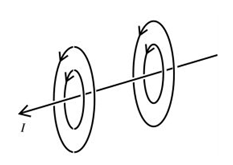
\includegraphics[width=6cm, height=4cm]{images/Capitulo_1/Campo_magnetico_en_un_conductor_sencillo}
	\caption{\textit{Campo magnético en un conductor sencillo.}}
	\label{fig:system:example1}	
\end{center}
\end{figure}
%\vspace*{3cm}
En el mismo año y de manera independiente Ampere dedujo que las cargas en movimiento eran las causas del campo magnético después de enterarse de los experimentos de Oersted. De acuerdo con la ley de ampere el campo magnético generado por un circuito eléctrico depende de la forma del circuito (trayectoria de conducción) y la corriente conllevada. Asumiendo que cada circuito esta echo de un número finito de elementos de corriente, cada uno contribuyendo al campo, integrando estas contribuciones en un punto para determinar el campo ampere concluyo que\\
\begin{equation}
	 \oint {\overrightarrow{H} \cdot d \overrightarrow{l}} =  I_{enc}
\end{equation}

\subsection{Inducción Magnética}
Cuando un campo magnético  H es generado por una corriente, de acuerdo a la ley de ampere,  la respuesta del medio es la inducción magnética B, también llamada densidad de flujo. Todos los medios responden con alguna inducción, en el vacío la relación entre el campo magnetizante y la inducción es \\ 	
						%inserte 3 formula%
Donde  $\mu$0 es la permeabilidad magnética del vacío, un constante universal cuyo valor es de $4\pi\times10^{-7}$

\subsection{Flujo Magnético}

¿Cómo podemos demostrar la presencia de un campo magnético?
Siempre que un campo magnético está presente, existirá un flujo magnético $ \phi$, este flujo y su razón de cambio pueden ser medidos ya que genera una fuerza electromotriz (f.e.m.) en un circuito conductor a través del cual pasa este flujo. Pequeñas partículas como el hierro se alinean con la dirección del flujo. La cantidad de flujo producido depende de las propiedades del medio y varía de un medio a otro.
\begin{equation}
	\phi = \int_{s}^{} \overrightarrow{H} \cdot d \overrightarrow{s}
\end{equation}

El weber es la cantidad de flujo que al ser reducido uniformemente a cero en un segundo produce una f.e.m. de un volt a través de una vuelta de conductor en la que atraviesa tal flujo.
\begin{figure}[htb]
\begin{center}
\centering
	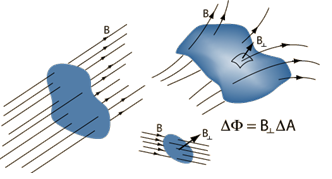
\includegraphics[width=6cm, height=4cm]{images/Capitulo_1/Flujo_magnetico}
	\caption{\textit{Flujo magnetico}}
	\label{fig:system:example1}	
\end{center}
\end{figure}

\section{Materiales Magnéticos}
\label{sec:related:sec3}
\subsection{Magnetización}

En muchos medios $B$ es una función lineal de $H$, en particular se puede decir que $B=\mu_0 H$, Si el valor de $B$ en el vacío es conocido entonces H puede ser inmediatamente calculado.
Sin embargo en otros medio, particularmente materiales ferromagnéticos, $B$ no es una fusión lineal d $H$, ni posee un mismo valor de $H$ para uno de $B$.
Ahora consideramos los efectos que un material tiene sobre la inducción magnética $B$ cuando un campo magnetizaste pasa a través de él. Esto está representado por la magnetización, ente pude ser incrementado en los ferromagnético, o ser reducido como en caso de los diamagnéticos. La permeabilidad relativa del material indica cómo cambia la inducción en el material comparada con la inducción en el vacío.\\\\\\

\begin{figure}[htb]
\begin{center}
\centering
	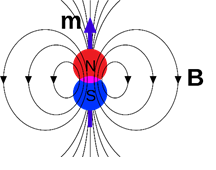
\includegraphics[width=6cm, height=4cm]{images/Capitulo_1/Dipolo_magnetico_de_un_atomo}
	\caption{\textit{Dipolo magnético de  un átomo}}
	\label{fig:system:example1}	
\end{center}
\end{figure}

Para el análisis de materiales magnético es necesario definir cantidades que representen la respuesta de estos materiales ante un campo magnético, estas cantidades son el momento magnético y la magnetización. Una vez que se ha hecho es posible considerar otra propiedad, la susceptibilidad, que está relacionada con la permeabilidad.
Se define una nueva cantidad $M$ (magnetización) como el momento magnético por unidad de volumen
\begin{equation}
	M = \frac{dm}{dV}
\end{equation}

A partir de la relación entre el momento magnético $m$ y el flujo se puede relación $M$ y $B$. Una barra magnética con una densidad $\phi$ en el centro, una longitud de dipolo de l y una área transversal A tiene un momento magnético de $m =\phi \mu_0$  , la magnetización  entonces está dada por $M = \frac{m}{Al}$. Entonces
\begin{equation}
	M = \frac{\phi}{\mu_0A} = \frac{B}{\mu 0}
\end{equation}

En este caso ninguna corriente externa está presente para un campo magnetizante por $B = \mu_0 M$. Podemos ver que la magnetización $M$ y el campo magnetizante $H$ contribuyen a la densidad de flujo en maneras similares.  Ambos magnetización y campo magnético están presentes  entonces sus contribuciones pueden ser sumandos.

\begin{figure}[htb]
\begin{center}
\centering
	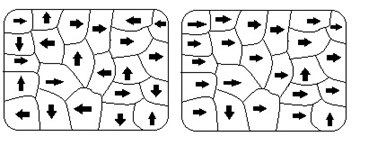
\includegraphics[width=10cm, height=4cm]{images/Capitulo_1/Dominios_magneticos_de_un_material}
	\caption{\textit{Dominios magnéticos de un material no magnetizado (izquierda) y uno magnetizado (derecha)}}
	\label{fig:system:example1}	
\end{center}
\end{figure}

\subsection{Permeabilidad y Susceptibilidad Magnética}

Los diferentes tipos de materiales magnéticos son clasificados de acuerdo a su susceptibilidad y permeabilidad. Entonces debemos de definir estos propiedades antes de describir diferencias entre materiales ferromagnéticos, paramagnéticos y diamagnéticos.
Para materiales isótropos y homogéneos la permeabilidad está definida como:
\begin{equation}
	\mu = \frac{B}{H}
\end{equation}

La susceptibilidad como:

\begin{equation}
	X=\frac{M}{H}
\end{equation}

Dado que $B$ y $M$ pueden o no ser una función lineal de $H$, dependiendo del tipo de material o medio debe de recalcarse que la permeabilidad y susceptibilidad podrían no ser constantes.\\
Es común usar el término permeabilidad relativa $\ mu_r$ definido como:
\begin{equation}
	\mu_r = \frac{\mu }{\mu_0}
\end{equation}

La permeabilidad relativa está relacionada con la susceptibilidad y la siguiente relación siempre es válida:
\begin{equation}
	\mu_r= X+1
\end{equation}

Y su relación con la inducción magnética de la forma:

\begin{equation}
	B=\mu_0 (H + M)
\end{equation}

Los diferentes materiales magnéticos son clasificados de acuerdo a su susceptibilidad. El primer grupo son los materiales  en los que $X$ es pequeña y negativa. Estos materiales son llamados diamagnéticos, su respuesta magnética se opone al campo magnético aplicado. Ejemplos de estos materiales son el cobre, plata, oro.  La superconductores forma otros grupo de diamagnéticos para los cuales $X=-1$.\\
Un segundo grupo de materiales en los que $X$ es pequeña y positiva son los materiales paramagnéticos. La magnetización de los materiales paramagnéticos es débil y alineada con la dirección del campo magnetizante, ejemplos de materiales paramagnéticos son el aluminio, platino y manganeso.\\
A temperatura constante y valores de campo $H$ relativamente bajas la susceptibilidad de los materiales diamagnéticos y paramagnéticos son contantes.

\begin{figure}[htb]
\begin{center}
\centering
	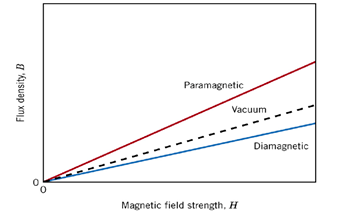
\includegraphics[width=11cm, height=7cm]{images/Capitulo_1/Curva_de_magnetizacion}
	\caption{\textit{Curva de magnetización para materiales paramagnéticos y diamagnéticos con respecto al vacío}}
	\label{fig:system:example1}	
\end{center}
\end{figure}

Los materiales magnéticos más prominentes son los ferromagnetismo, cuya susceptibilidad es positiva y mucho mayor a 1, con valores típicos de $X$ entre los 50 a 10000. Ejemplos de estos materiales son el hierro, cobalto níquel, metales de tierras raras y sus aleaciones.

\subsection{Saturación}
¿Existe un límite para magnetización de un material?
Si un material tiene n dipolos atómicos por unidad de volumen una vez que todos estos dipolos quedan alineados en paralelo se alcanza la magnetización de saturación $M_0$. Se puede realizar una distinción entre la saturación técnica $M_s$  y la saturación Completa $M_0$. 

\begin{figure}[htb]
\begin{center}
\centering
	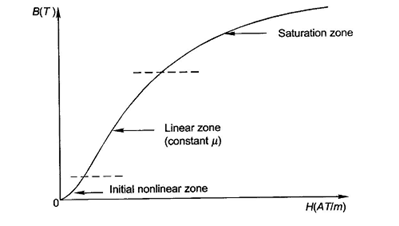
\includegraphics[width=11cm, height=7cm]{images/Capitulo_1/Curva_de_magnetizacion_de_un_material_ferromagnetico}
	\caption{\textit{Curva de magnetización de un material ferromagnético.}}
	\label{fig:system:example1}	
\end{center}
\end{figure}

\subsection{Histéresis}

\begin{figure}[htb]
\begin{center}
\centering
	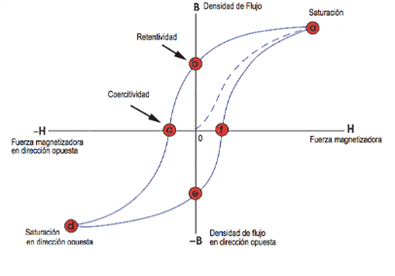
\includegraphics[width=11cm, height=7cm]{images/Capitulo_1/Curva_de_histeresis}
	\caption{\textit{Curva de histéresis.}}
	\label{fig:system:example1}	
\end{center}
\end{figure}

Los efectos de histéresis añaden más complicaciones debido a que la magnetización M  del material depende no solo del campo magnético H como del historial de magnetización del material. Incluso en los casos donde la histéresis ocurre métodos han sido creados para los cálculos de los campos magnéticos en estos dispositivos, en donde la histéresis se tiene en cuenta.

\subsection{Remanecía}

¿Qué le sucede a la inducción magnética de un material ferromagnético una vez que fuerza magnetizante es retirada?\\
Una vez que campo magnetizante es reducido a cero después de magnetizar un material ferromagnético permanece un porción residual de magnetización y por consiguiente una inducción residual donde
\begin{equation}
	B_R=\mu_0 M_R
\end{equation}

En una convención emergente se hace una distinción entre remante y remanencia, donde la remanencia es usada para describir el valor residual de la magnetización después haber llevado el material a saturación, mientras que la magnetización remanente  se refiere al valor residual después de magnetizar el material en un nivel arbitrario.

\subsection{Coercitividad}

La inducción magnética puede ser reducida a cero después de aplicar un campo magnetizante inverso de magnitud $H_c$. Esta intensidad de campo es conocida como coercitividad. Es fuertemente dependiente de la condición de la muestra, siendo afectada por factores como tratamientos térmicos y deformaciones.\\
La coercitividad intrínseca está definida como la intensidad de campo para la cual la magnetización es reducida a cero, en materiales ferromagnéticos suaves $H_c$ y $H_{ci}$ tiene un valor cercano, mientras que en materiales duros está clara una diferencia entre ellas con $H_{ci}$ siendo siempre mayor que $H_c$.

\subsection{Temperatura de Curie}

¿Qué sucede cuando un material ferromagnético es calentado?
Cuando los materiales ferromagnéticos son calentados a temperaturas lo suficientemente altas se convierten en materiales paramagnéticos. La temperatura de transición entre ferromagnetismo y paramagnetismo es ferromagnetismo es conocida como temperatura de Curie. A esta temperatura la permeabilidad de material baja súbitamente y ambas coercitividad y remanencia se vuelven cero.

\subsection{Materiales Ferromagnéticos}

Podemos clasificar los materiales ferromagnéticos en base a su coercitividad. La coercitividad es un propiedad magnética dependiente de la estructura,  esto significa que se puede altera sometiendo al espécimen a diferentes tratamientos térmicos y mecánicos.\\
Fue descubierto que los materiales de a base de hierro con alta dureza mecánica también presentaban una alta coercitividad, mientras que aquellos materiales más maleables tenían una coercitividad menor. Por lo tanto los términos suaves y duros fueron usados para distinguir los materiales ferromagnéticos de acuerdo a esta propiedad. Los materiales duros poseen  una coercitividad sobre los $10K \frac{A}{M}$ mientras aquellos con una coercitividad menor a  $1k \frac{A}{m}$ son considerados suaves.\\
La selección de un material ferromagnético será determinada por las características mostradas en sus lazos de histéresis. Materiales para transformadores necesitan una alta permeabilidad y baja histéresis debido a la necesidad de una alta eficiencia en la conversión de energía eléctrica. Los electroimanes requieren una baja coercitividad y remanencia para reducir fácilmente la magnetización a cero durante el apagado. Finalmente los imanes permanentes requieren de una alta remanencia y coercitividad para retener la mayor magnetización posible. 

\subsection{Aplicaciones de los Materiales Ferromagnéticos}

Electroimánes\\
¿Dónde se usan los materiales ferromagnéticos?
Los materiales ferromagnéticos suaves son usados en electroimánes, motores, transformadores, y relés. Materiales usados en el núcleo de los electroimánes deben de tener una alta permeabilidad, permitiendo alcanzar una lata inducción magnética, al mismo tiempo debe poseer una baja coercitividad de manera que la inducción magnética pueda ser fácilmente revertida.\\
Imanes permanentes\\
¿Dónde usamos materiales ferromagnéticos que quedan permanentemente magnetizado?
Los imanes permanentes son una de las clases más importantes de materiales magnéticos, otros siendo los aceros eléctricos y los imanes de grabación. Los imanes permanentes tienen aplicación in motores eléctricos y generadores, parlantes, televisiones, galvanómetros, dispositivos de suspensión magnética.\\
Para estas aplicaciones el material se  determina a partir de sus histéresis, como la coercitividad y remanencia, es importante resaltar que estas propiedades magnéticas dependen fuertemente de los tratamientos a los que fue sometido el material.\\
En años recientes materiales para imanes permanentes basados en neodimio-hierro-boro han sido descubiertos,  por ejemplo su coercitividad puede ser tan alta como $1.12x106 A/$, comparada con $0.72\times 106$ para samario-cobalto.\\
Además de la coercitividad otro parámetro de vital importancia es el producto energético $BH_{max}$, este es obtenido mediante el producto máximo $BH$ en el segundo cuadrante  de la curva de histéresis,  Este representa la energía magnética almacenada en el material y es usualmente especificado por los fabricantes de imanes permanentes.

\section{Análisis de Circuitos Magnéticos}
\label{sec:related:sec3}

Situaciones en las que la trayectoria del flujo magnético esta interrumpida por un espacio libre (entrehierro) son de gran importancia para las aplicaciones ingenieriles de imanes permanentes, motores, generadores y demás maquinarias eléctricas. \\
Los problemas encontrados aquí son más complicados que  calcular el flujo en un solo material, sin embargo algunas simplificaciones a las ecuaciones de flujo magnético y campo magnetizante pueden usarse para encontrar soluciones a estos problemas.\\
Realizando simplificaciones a partir de las ecuaciones de maxwell, comenzando por la ley de gauss magnética, donde se establece la conservación del flujo magnético alrededor de un nodo.\\
\begin{equation}
	 \oint {\overrightarrow{B} \cdot d \overrightarrow{s}} = 0 \Rightarrow \phi_1 +\phi_2 ... + \phi_i = 0
\end{equation}

La fuerza magnetomotriz $\eta$ como la excitación magnética
\begin{equation}
	Ni = \oint {\overrightarrow{H} \cdot d \overrightarrow{l} = \eta}
\end{equation}

La reluctancia magnética $R$ dependiente de la geometría y material de la muestra
\begin{equation}
	R = \frac{l}{\mu A}
\end{equation}

Y finalmente la relación entre estas, también conocida como ley de Hopkinso

\begin{equation}
	\phi = \frac{\eta}{R}
\end{equation}

\begin{figure}[htb]
\begin{center}
\centering
	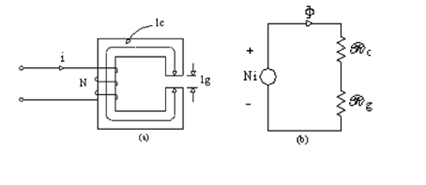
\includegraphics[width=11cm, height=7cm]{images/Capitulo_1/Elementos_de_un_circuito_magnetico}
	\caption{\textit{Elementos de un circuito magnético.}}
	\label{fig:system:example1}	
\end{center}
\end{figure}

A partir de estas ecuaciones es posible el sencillo cálculo del flujo a través de  elementos con diferentes longitudes medias, materiales y secciones transversales mediante las técnicas de análisis de circuitos eléctricos mediante las analogías:\\\\

\begin{tabular}{|c|c|c|c|}
\hline 
Circuitos magnéticos &  & Circuitos eléctricos &   \\ 
\hline
$\eta$ & Fuerza magnetomotriz & $\varepsilon$ & Fuerza electromotriz \\ 
\hline 
$\phi$ & Flujo magnético & $I$ & Corriente eléctrica \\ 
\hline 
 $R$ & Reluctancia & $r$& Resistencia eléctrica\\
\hline
\end{tabular} 

\section{Caracterización de Materiales}
\label{sec:related:sec3}

Para el diseño de electroimánes se requiere conocer las características magnéticas del material, como la permeabilidad relativa y el punto de saturación, sin embargo lo materiales ferromagnéticos comercializados localmente carecen de hojas de especificaciones de donde obtener esta información por lo es necesario disponer de un método para caracterizar sus propiedades más relevantes.

\subsection{Análisis}

A partir de la ley de Faraday que relaciona la variación temporal del flujo eléctrico y la fuerza electromotriz inducida
\begin{equation}
	\varepsilon =\frac{d \lambda}{dt} = \frac{N d \phi}{dt}
\end{equation}

La ley de ampere:
\begin{equation}
	\oint {\overrightarrow{H} d \overrightarrow{l}} = HL = NI \Rightarrow H = \frac{NI}{L}
\end{equation}

Y el concepto de permeabilidad diferencial [cita a la definición de permeabilidad diferencial:
\begin{equation}
	\mu_d = \frac{dH}{dt}
\end{equation}

Es posible obtener una relación entre variables eléctricas medibles (corriente y voltaje)  y la permeabilidad relativa de un núcleo cerrado de longitud promedio L, sección transversal A y N espiras en su embobinado:

\begin{equation}
	\frac{d \phi}{dt} = \frac{d \phi dB}{dB dt} = A \frac{dB}{dt}
\end{equation}
\begin{equation}
	\frac{dB}{dt} = \frac{dB dH}{dH dt} = \mu_d \frac{dH}{dt}
\end{equation}
\begin{equation}
	\frac{dH}{dt} = \frac{dH dI}{dH dt} = \frac{N dI}{L dt}
\end{equation}
\begin{equation}
	\varepsilon = \mu_d (\frac{N^2 A}{l} \frac{dI}{dt})
\end{equation}
\begin{equation}
	\mu_d= \frac{\frac{\varepsilon}{dI}}{dt} (\frac{L}{N^2 A})
\end{equation}

Mediante las mediciones de corriente y voltaje en la bobina se calcula la permeabilidad diferencial para cada punto de I y lo tanto para cada punto de $H$, después de la  integrar la función obtenida $\mu_d (H)$  se puede obtener un aproximado de $B$:
\begin{equation}
	B = \int dB = \int \mu_d dH
\end{equation}

\section{Electroimánes}
\label{sec:related:sec3}
\subsection{Análisis del Electroimán}	

Mediante el análisis de circuitos magnéticos se puede calcular la energía almacenada en el circuito formado por el electroimán.
\begin{figure}[htb]
\begin{center}
\centering
	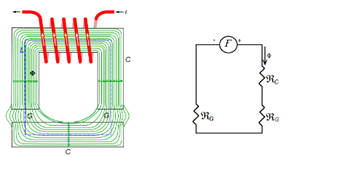
\includegraphics[width=11cm, height=7cm]{images/Capitulo_1/Circuito_magnetico_del_electroiman}
	\caption{\textit{Circuito magnético del electroimán.}}
	\label{fig:system:example1}	
\end{center}
\end{figure}

\begin{equation}
	W_m = \frac{1}{2} Li^2 = \frac{\mu_0 N^2 I^2 A}{2 (\frac{l_e}{\mu_{re}}+ \frac{l_a}{k \mu_{ra}}+ 2y)^2}
\end{equation}

Aplicando el principio de trabajo virtual podemos calcular la fuerza como le variación de la energía con respecto al despeamiento.
\begin{equation}
	F_m = \frac{dW_m}{dy} = - \frac{\mu_0 N^2 I^2 A}{(\frac{l_e}{\mu_{re}}+ \frac{l_a}{k \mu_{ra}}+ 2y)^2}
\end{equation}

Suponiendo que flujo es uniforme sobre la sección transversal núcleo es posible calcular la inducción magnética del material

\begin{equation}
	B = \frac{\phi}{A} = \frac{\mu_0 NI}{\frac{l_e}{\mu_{re}}+\frac{l_a}{k \mu_{ra}+2y}}
\end{equation}

Estas ecuaciones resultan difíciles de trabajar para el diseño del electroimán, sin embargo en el caso de que la condición
\begin{equation}
	u_{r,}y \bracevert 2y >>\frac{l_e}{\mu_{re}} + \frac{l_a}{k \mu_{ra}}
\end{equation}

Sea válida, Los términos que dependen de las longitudes del conductor magnético se vuelven despreciables y las ecuaciones se simplifican a
\begin{equation}
	F_m = - \frac{\mu_0 N^2 I^2 A}{4y^2}
\end{equation}
\begin{equation}
	B = \frac{\mu_0 N I}{2y}
\end{equation}
Gracias a la alta permeabilidad de la ferrita y las condiciones de operación $y_min$   y  $y_max$ estas ecuaciones pueden ser usadas para el cálculo del electroimán.

\section{Imán Permanente}
\label{sec:related:sec3}
\subsection{Análisis del Imán Permanente}

Proponiendo un imán permanente y guía de flujo magnético con la siguiente geometría:
\begin{figure}[htb]
\begin{center}
\centering
	
	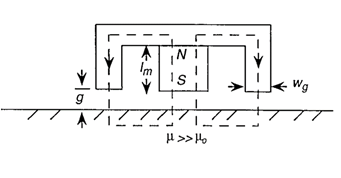
\includegraphics[width=5cm, height=5cm]{images/Capitulo_1/Circuito_magnetico_de_iman_permanente}
	\caption{\textit{Circuito Magnético de imán permanente.}}
	\label{fig:system:example1}	
\end{center}
\end{figure}

\begin{figure}[htb]
\begin{center}
\centering
	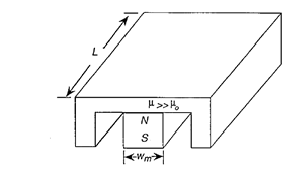
\includegraphics[width=5cm, height=5cm]{images/Capitulo_1/Geometria_de_iman_y_ferrita_guia}
	\caption{\textit{Geometria de imán y ferrita guia.}}
	\label{fig:system:example1}	
\end{center}
\end{figure}

Asumiendo que el plato tiene una permeabilidad relativa infinita y que el imán posee una curva de demagnetización lineal de la forma:
\begin{equation}
	B_m = B_r + \mu_rH_m
\end{equation}

Teniendo en cuenta la falta de fuerza magnetomotriz:

\begin{equation}
	H_m l_m +2Hg = 0 
\end{equation}

Y finalmente la conservación de flujo magnético:
\begin{equation}
	B_m A_m = 2B_g A_g
\end{equation}

Podemos calcular la inducción magnética en el entrehierro:

\begin{equation}
	  B_g(g) = (\frac{A_m}{A_g}) \frac{B_r}{2(1+(\frac{\mu_m}{\mu_0})(\frac{A_m}{A_g})(\frac{g}{l_m}))} 
\end{equation}

Y por consiguiente la fuerza aplicada por el imán permanente debido a una variación en la energía aplicada en el entrehierro.
\begin{equation}
	F_g(g)= \frac{1}{2} \mu_0  \oint \oint B_g^2 ds \hat{n}
\end{equation}
\begin{equation}
	F_g(g)= \frac{1}{2 \mu_0} (2B-^2(g)A_g +B_m^2A_m)  \hat(n)
\end{equation}
\begin{equation}
	F_g(g) = \frac{B_r^2}{2 \mu_0 (1 + (\frac{\mu_m}{\mu_0})(\frac{A_m}{A_g})(\frac{g}{l_m}))^2}[\frac{A_m + 2A_g}{2Ag}] \hat{n}
\end{equation}

Donde
\begin{enumerate}
	\item $A_m$: Es la sección transversal del imán permanente
	\item $A_g$: La sección transversal del entrehierro
	\item $l_m$: La longitud media del imán permanente
	\item $B_r$: La inducción remanente
	\item $H_c$: La coercitividad
	\item $\mu_m$: La permeabilidad magnética del imán permanente definida como  $\frac{B_r}{H_c}$
	\item:$g$ La distancia de entrehierro

\end{enumerate}

\section{Sensores de Desplazamiento}
\label{sec:related:sec3}
\subsection{Requerimientos del Sensor}

Las condiciones de operación del sensor presentan dificultades incluyendo:
\begin{enumerate}
	\item Un rango de operación reducido (1mm a 3mm)
	\item Medición sin contacto 
	\item Inmunidad al ruido de acoplamiento magnético causado por los electroimanes
	\item Rápida respuesta
	\item Resolución mínima  100$um$

\end{enumerate}

\subsection{Tipos de Sensores}
La mayoría de los sensores de desplazamiento de alta precisión requieren de contacto directo como los encoders de cuadratura, potenciómetros y sensores LVDT (Linear Variable Differential Transformer).\\
Los sensores que no requieren de directo con el objeto se basan en la transformación de energía (transductores) o en la medición de alguna propiedad fundamental (resistencia, capacitancia, inductancia) para la detección de esa distancia.\\
Entre los sensores de tipo transductor encontramos los sensores ultrasónicos que:
\begin{enumerate}
	\item Emiten ondas sónicas de alta frecuencia
	\item Las ondas viajan hasta el objeto a detectar y son reflejadas sobre su superficie (siempre y cuando las características del material lo permitan en mayor o menor medida) 
	\item Las ondas reflejadas son detectadas y tiempo entre la transmisión de onda y la recepción es medido. Este tiempo es función directa de la distancia del objeto y la velocidad de propagación en el medio por que la distancia es calculada
\end{enumerate}

Estos sensores tienen la desventaja de poseer un rango mínimo de 10-20$cm$ y un rango máximo determinado por la potencia de la señal transmitida. Estas características. Además del tamaño del transductor no parecen ser una solución al problema de medición.\\
Otros sensores de operación similar son los sensores de tipo “time of fligth” (tiempo de vuelo), estos operan emitiendo un haz de luz no visible en lugar de ondas ultrasónica, poseen un rango reducido, su resolución es baja y su tiempo de respuesta es lento.\\
Los inductivos son especialmente útiles para la detección de materiales metálicos y ferromagnéticos pero debido a la presencia de un campo variable generado los electroimanes adyacentes sus mediciones podrían presentar errores debido a la interferencia.\\

Por otro lado los sensores capacitivos presentan una alta resolución, rango reducido y una detección de objetos no aterrizados y sin contacto siempre y cuando el objeto posea una permitividad mayor a la del vacío, además de poseer una respuesta ultrarrápida.

\subsection{Sensores de Desplazamiento Capacitivo}
A continuación se describen las propiedades básicas de la tecnología de sensores capacitivos y sus aplicaciones industriales. 
Características de los capacitores\\
Los capacitores son el bloque de construcción en el mundo electrónico. Para entender cómo operan estos sensores es importante entender las propiedades y principios fundamentales de los capacitores. Esta sección describe los aspectos físicos, geométricos, y eléctricos de los capacitores.\\
Los capacitores son dispositivos que consisten en dos electrodos separados por un aislante, los capacitores generalmente se componen de dos placas conductivas separadas por un material no conductivo llamado dieléctrico. La energía eléctrica o carga es almacenada en estas placas. \\
Una vez que un voltaje es aplicado a través de las terminales del capacitor los platos conductivos comenzaran a almacenar energía electica hasta que la diferencial de potencial entre estas iguale al voltaje aplicado por la fuente de voltaje.
La carga eléctrica permanece en las palcas incluso después de desconectar la fuente de voltaje a menos que otro componente consuma esta carga o el capacitor se descargue a cusa de las fugas de corriente debido la imperfecciones del aislante dieléctrico.
Sensores de desplazamiento capacitivos\\
Un sensor de capacitivo convierte el cambio eléctrico entre dos conductores en una señal eléctrica. Los sensores se construyen variando algunos de los parámetros que influyen en la capacitancia que según  la ecuación  de capacitancia entre placas paralelas serian el área, la distancia entre placas  o la permitividad del dieléctrico.
$C=F(d,A,\varepsilon_r)$\\
Un sensor de proximidad es un transductor que es capaz de detectar la presencia de un objeto sin contacto físico, normalmente un sensor de proximidad emite alguna campo electromagnético o electrostático, o un haz de radiación electromagnética (radiación infrarroja) y detecta cualquier cambio en el campo o señal de retorno. Sensores de proximidad capacitivo consisten en un oscilador cuya frecuencia está determinada por la capacitancia del circuito al cual los electrodos están conectados, cuando un conductor aterrizado o un material con una alta permeabilidad electica se acercan al electrodo la capacitancia cambia la frecuencia del oscilador. Este cambio es detectado y enviado a la unidad de control. El objeto detectado se le refiere comúnmente como objetivo.
El campo eléctrico distribuido alrededor del capacitor experimenta un cambio el cual es detectado por la unidad de control.

\begin{figure}[htb]
\begin{center}
\centering
	
	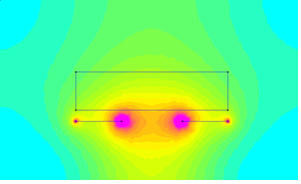
\includegraphics[width=5cm, height=5cm]{images/Capitulo_1/Interaccion_del_campo_electrico_en_un_capacitor_aire}
	\caption{\textit{Interacción del campo eléctrico en un capacitor de placas coplanarias con espacio frontal relleno de aire .}}
	\label{fig:system:example1}	
\end{center}
\end{figure}

\begin{figure}[htb]
\begin{center}
\centering
	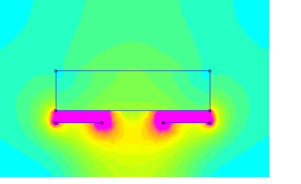
\includegraphics[width=5cm, height=5cm]{images/Capitulo_1/Interaccion_del_campo_electrico_en_un_capacitor_aire_dielectrico}
	\caption{\textit{Interacción del campo eléctrico en un capacitor de placas coplanarias con espacio frontal relleno de dieléctrico.}}
	\label{fig:system:example1}	
\end{center}
\end{figure}

La distancia máxima que el sensor de proximidad es capaz de detectar es conocido como rango nominal. Algunos sensores tienen ajustes del rango nominal o maneras de reportar una detección graduada de la distancia, un sensor de proximidad ajustado a un rango muy limitada es comúnmente referido como un sensor táctil. Los sensores capacitivos usualmente tienen el doble de rango los sensores inductivos.\\



Susceptibilidad a capacitancias parasitas
Los electrodos del sensor poseen capacitancias en el rango de fracción de picofaradios y conectar esas señales a un cable coaxial de 60pF por metro podría obscurecer totalmente la señal. Sin embargo con el blindaje correcto al igual que cualquier otra capacitancia parasita es posible eliminar en mayor medida los efectos  del ruido.
Susceptibilidad al ruido\\
Un peligro para los circuitos osciladores  es que la frecuencia variaría de manera intermitente en el caso de existiría interferencia cruzada causada por circuitos adyacentes, estos problemas pueden ser resueltos mediante un blindaje, una correcta disposición de pistas e integrados en el circuito y el  uso de capacitores de “bypass” en las fuentes de alimentación.\\
Distancia entre los electrodos\\
La capacitancia depende del entrehierro o distancia entre los electrodos conductivos. Esta distancia pude incrementar o decrementar dependiendo de las condiciones ambientales, y del material que podrían generar un mediciones poco exactas, por ejemplo suciedad en la superficie del sensor.



\section{Modelado dinamico, control y simulacion}

Ahora que diseñamos los sensores y actuadores podemos continuar con el modelado dinamico del eje y el control.
A cotinuacion se presenta:
\begin{itemize}
\item El modelo dinamico del rotor
\item La linearizacion del modelo dinamico
\item El diseño de various esquemas de control
\item El algoritmo final de control
\end{itemize}


\subsection{Modelado dinamico}
\subsection{Conceptos de sistemas}
Un sistema es un objeto o proceso en el cual se tiene al menos una entrada y una salida bien definidas. Estos suelen representarse mediante un bloque mostrando sus respectivas entradas y salidas.  

\begin{figure}
\begin{center}
\centering
\missingfigure[figwidth=6cm]{Diagrama de bloque de un sistema}
\caption{Representacion de bloque de un sistema}
\end{center}
\end{figure}

Un sistema que responde a un entrada con una salida, unicamente pdespues de que esta fue aplicada es conocido como causal.
Lo que se busca en el modelado es, a partir de un conjunto de un 
conjunto de leyes fisicas llegar a un sistema de ecuaciones diferenciales que despues 
seran de ayuda para diseñar un control adecuado. Debido a la naturaleza mixta del 
sistema, las ecuaciones resultantes incluiran terminos tanto del dominio mecanico como 
del dominio electromagnetico. Posteriormente este conjnto de ecuaciones no lineales seran linearizadas con fin de aprovechar las tecnicas de control moderno.


\subsection{Sistemas dinamicos}
Un sistema es cualquier proceso o 

En parte se pueden clasificar como:
\begin{itemize}
\item lineales o no lineales
\item Deterministicos o Estocasticos
\item Variantes o invariantes en el tiempo
\end{itemize}

\subsection[1]{LTI}
Los sistemas lineales invariates en el tiempo (LTI por sus siglas en ingles) son sistemas que tienen una ecuacion diferencial de la forma


%%$$ a_n\frac{d^ny}{dt^n} + a_n-1\frac{d^n-1y}{dt^n-1} 
%%+ a_1\frac{dy}{dt} +a_0y+ = F$$
Este tipo de ecuaciones tienen co
\subsection{Dinamica de una particula}

Ley de Newton
La ley de newton establece que 
$$ \vec{F} = m\vec{a} $$
para una masa puntual con grado de libertad esta equacion puede
escribirse como
$$ \frac{d^2x}{dt^2}=\frac{F(t,x)}{m}$$
la cual es una ecuacion diferencial de segundo grado donde la fuerza puede ser una
funcion dependiente de la posicion $x$ y del tiempo $t$.
Donde $F$ es el conjunto de fuerzas que actuan sobre la particula, si estas fuerzas pueden ser representadas como una combinacion lineal de derivadas de la posicion $x$ de la forma.

\subsection{Dinamica de un cuerpo rigido}

Momento de inercia

Torque y aceleracion angular

Ecuaciones de euler

Precesion
\subsection{Integrando los electroimanes}
\subsection{Linearizacion}
\section{Control}
\subsection{Control retroalimentado}
\subsection{Control integral}
\subsection{Control calendarizado}
\subsection{Discretizacion de controladores}
\subsection{Accionamiento hibrido}

   % INCLUDE: related work

%\part{Additional Example Part}
% !TEX root = ../thesis-example.tex
%
\chapter{Diseño Conceptual}
\label{sec:system}

\cleanchapterquote{La absoluta inspiración es la fecha límite.}{Nolan Bushnell}{(Fundador Atari, Inc.)}


\section{Necesidad}
\label{sec:system:sec1}

Los ejes de transmisión de las máquinas se encuentran sometidos constantemente a la fricción y a las vibraciones producto del contacto que existe entre estos y las piezas a las que estén conectados. Esto conlleva una serie de problemas como el aumento de la temperatura de operación y el desgaste de las piezas. Para disminuir estos efectos es necesaria la utilización de cojinetes o rodamientos sobre los que se sostengan y giren los ejes de transmisión.  

Algunas de estas máquinas requieren operar a un alto régimen de revoluciones, y para ello se han desarrollado los rodamientos magnéticos, los cuales generan un campo magnético que ayuda al eje de transmisión a permanecer en un estado de levitación, suprimiendo el contacto directo que tendría con un cojinete o rodamiento convencional y facilitando el giro del eje. Esto implica una disminución de la temperatura de operación, las vibraciones y el ruido, así como la posibilidad de reducir la potencia de los motores y los costos de mantenimiento relacionados al remplazo de piezas por desgaste y a la utilización de lubricantes. 

La mayoría de los rodamientos magnéticos desarrollados han sido de tipo activo, por lo que utilizan electroimánes para generar el campo magnético. El problema con esto es que requieren un constante suministro de energía eléctrica, lo que implica un incremento en el consumo de energía de la máquina en comparación con utilizar cojinetes convencionales. 

Es por ello que es necesario buscar una alternativa que pueda dar solución a este problema. El rodamiento magnético híbrido utiliza un imán permanente para generar un campo magnético base de levitación que mantendrá al eje en su posición una vez que los electroimánes lo hayan estabilizado, por lo que no requieren estar operando de forma permanente. 

\section{Especificaciones de Diseño del Producto (PDS)}
\label{sec:system:sec2}

Para delimitar los requerimientos de diseño se hace uso de una herramienta denominada PDS (por sus siglas en inglés Product Design Specifications). Esta herramienta documenta las características del producto y define las especificaciones y restricciones de diseño; dichas especificaciones permanecen en constante evolución a lo largo del proyecto, con base en la información adquirida a lo largo del desarrollo y las modificaciones que se consideren pertinentes.  
A continuación, se enlistan las especificaciones de diseño de los Rodamientos Magnéticos Híbridos:

\begin{itemize}
\addtolength{\itemsep}{-1mm}
\item Desarrollarse bajo una estructura lo más compacta posible sin sacrificar la funcionalidad.
\item Considerar el uso de materiales y componentes asequibles y con disponibilidad en el mercado. 
\item Capaz de soportar una carga estática de 1kg.
\item Considerar un diseño por módulos funcionales. 
\item Contar con un dispositivo mecánico de seguridad que sostenga el rotor en caso de que el sistema no se encuentre energizado.
\item Simplificación de las operaciones de ensamble. 
\item La levitación del rotor debe ser posible independientemente del material de fabricación de este. 
\end{itemize}



\section{Análisis Funcional}
\label{sec:system:sec3}

Una de las primeras consideraciones realizadas para el desarrollo del rodamiento magnético hibrido fue consolidar el diseño con base en módulos más sencillos que posteriormente pudieran integrarse para formar el sistema. Esta metodología es denominada Diseño Modular.
 
El diseño modular consiste en la creación de módulos funcionales, que unidos, forman estructuras mayores que pueden ser ensambladas de diferentes maneras o disposiciones; esta técnica tiene como finalidad que dichos módulos se puedan diseñar, desarrollar, probar y modificar de manera sencilla y lo más independientemente posible del resto del sistema. Esto simplifica en gran medida los procesos de manufactura y ensamble requeridos. 

Entre otras de sus ventajas podemos destacar:

\begin{itemize}[noitemsep]
\item Permite la planificación individual de los productos.
\item En caso de presentarse alguna falla, basta con determinar el módulo del que procede y realizar las reparaciones. 
\item Reduce los tiempos y costes de mantenimiento.
\end{itemize}

Con base en estos principios, se realizó la descomposición del rodamiento magnético híbrido en los siguientes módulos:

\begin{itemize}
%\begin{enumerate}[(a)]
\item Rodamiento magnético activo radial: genera el campo magnético para las cargas radiales por medio de electroimanes. 
\item Rodamiento magnético activo axial: genera el campo magnético para las cargas axiales por medio de electroimanes.
\item Arreglo de sensores de desplazamiento: miden la posición del rotor para realizar las correcciones necesarias para estabilizarlo. 
\item Módulo de compensación de cargas estáticas: provee un campo magnético base de levitación por medio de un imán permanente. 
\item Módulo de seguridad: consiste en un mecanismo que sea capaz de sostener y estabilizar el rotor cuando el sistema no se encuentre energizado, ya sea por acción del usuario o por un fallo en el suministro eléctrico. 
%\end{enumerate}
\end{itemize}

Cada uno de estos módulos cumple con una función específica, por lo que cuentan con características y requerimientos de operación particulares que hace posible que puedan diseñarse individualmente, pero al mismo tiempo son capaces de trabajar en conjunto y cumplir con la función principal del rodamiento magnético híbrido. 

Una vez que se ha determinado la división por módulos del sistema, se identifican las funciones o prestaciones que debe cumplir para cubrir la necesidad, y convertirlas en especificaciones de diseño.

A continuación se muestra el diagrama por áreas funcionales del rodamiento magnético híbrido, donde se aprecia cómo interactúan los módulos con el resto de los subsistemas:

\begin{figure}[htb]
\centering
	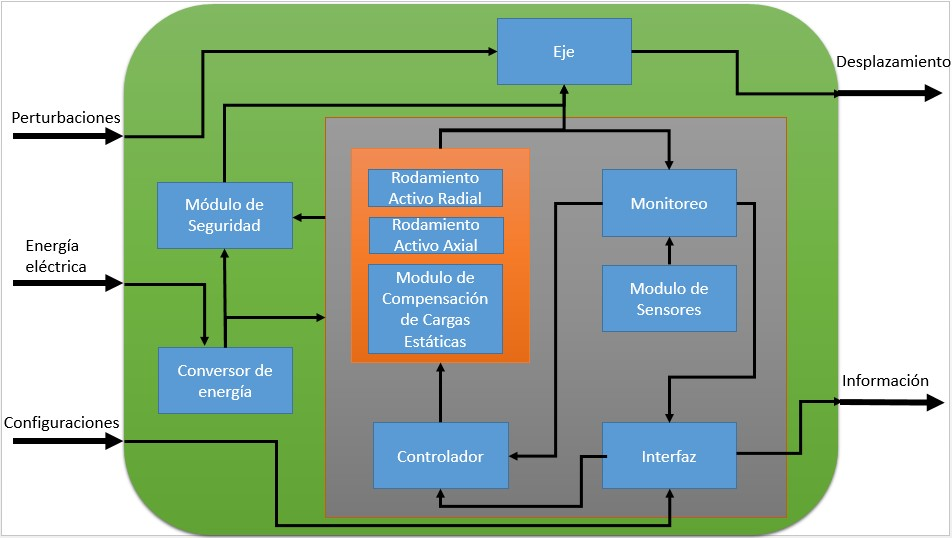
\includegraphics[width=\textwidth]{images/Capitulo_2/DiagramaFuncional}
	\caption{\textit{Diagrama Funcional.}}
	\label{fig:system:example1}
\end{figure}

Del diagrama de áreas funcionales podemos reconocer que el sistema cuenta con 2 entradas que determinan el funcionamiento y el comportamiento del mismo: el suministro de energía eléctrica y las perturbaciones que llegan al sistema. Este diagrama se divide en 3 secciones principales: la primera sección lo componen los módulos que generan los campos magnéticos de levitación, los cuales deben variar de acuerdo a lo que indique el controlador. Este se encuentra dominado por el monitoreo del módulo de sensores y la interfaz de usuario, la cual además muestra información sobre la posición del rotor. 

La tercera sección incluye el convertidor de energía que alimenta todos los sistemas eléctricos, incluyendo el módulo de seguridad, el cual se rige a través de la información que provea el controlador, ya que este sólo actúa con el corte del suministro eléctrico o por alguna falla detectada por el controlador. 


\section{Diseño Conceptual del Producto}
\label{sec:system:sec4}

La arquitectura del sistema fue planteada con base en la investigación teórica sobre las características generales de los rodamientos magnéticos y en la división por módulos funcionales, de manera que pudieran diseñarse individualmente. 

\subsection{Rodamiento Magnético Activo Radial}

Los rodamientos magnéticos activos utilizan un arreglo de electroimanes opuestos para generar los campos magnéticos de levitación, y están diseñados para soportar las cargas radiales que actúan sobre el rotor, manteniéndolo centrado sobre el eje de rotación de la máquina.

\begin{figure}[htb]
\centering
	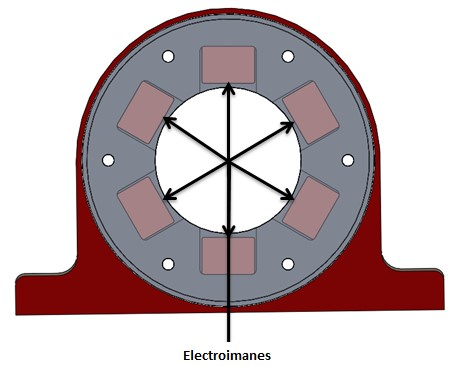
\includegraphics[scale=.65]{images/Capitulo_2/RMAR}
	\caption{\textit{Diseño conceptual del rodamiento magnético activo radial.}}
	\label{fig:system:example1}
\end{figure}

\subsection{Rodamiento Magnético Activo Axial}

Como su nombre lo dice, los rodamientos magnéticos axiales están diseñados para soportar cargas axiales. Estos utilizan un collar de soporte, el cual consiste por lo general en un disco plano, sólido, de material ferromagnético fijado al rotor. Los electroimánes en forma de disco están situados a cada lado del collar y sujetos a la carcasa de la máquina. Utilizan un sensor o arreglo de sensores que mide la posición del rotor en dirección axial. 

\begin{figure}[htb]
\centering
	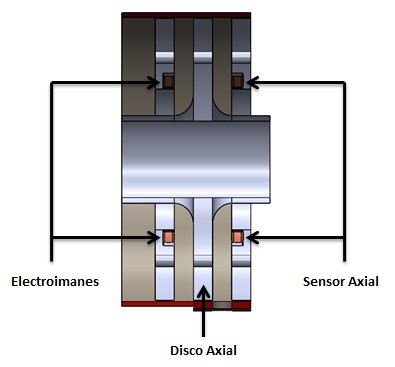
\includegraphics[scale=.65]{images/Capitulo_2/RMAA}
	\caption{\textit{Diseño conceptual del rodamiento magnético activo axial.}}
	\label{fig:system:example1}
\end{figure}

\subsection{Módulo de Sensores}

Este arreglo de sensores para el rodamiento magnético activo radial 
envía las señales de posición del rotor al controlador. El controlador utiliza esta información para modificar el campo electromagnético en el rodamiento.

\begin{figure}[htb]
\centering
	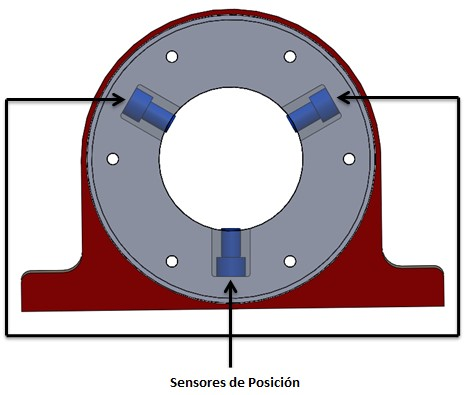
\includegraphics[scale=.65]{images/Capitulo_2/MS}
	\caption{\textit{Diseño conceptual del arreglo de sensores para los desplazamientos radiales.}}
	\label{fig:system:example1}
\end{figure}

%\clearpage

\subsection{Módulo de Compensación de Cargas Estáticas}

Este módulo se basa en el principio de funcionamiento de los rodamientos magnéticos pasivos. Utiliza un imán permanente para generar un campo magnético base de levitación que ayude a disminuir el consumo de energía del rodamiento magnético radial. Debe utilizar un mecanismo de desplazamiento que varíe la distancia entre el imán permanente y el rotor para ajustar el campo magnético. 

\begin{figure}[htb]
\centering
	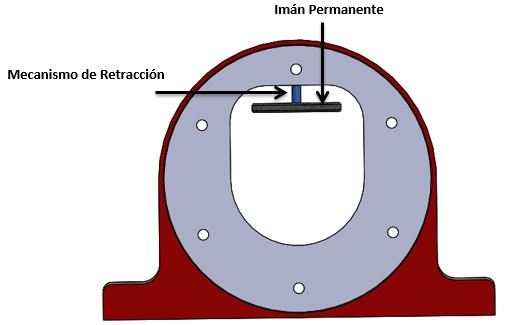
\includegraphics[scale=.70]{images/Capitulo_2/MCCE}
	\caption{\textit{Diseño Conceptual del módulo de compensación para cargas estáticas.}}
	\label{fig:system:example1}
\end{figure}

\subsection{Módulo de Seguridad}

Uno de los elementos más importantes con los que debe contar un rodamiento magnético es un mecanismo auxiliar que tenga como finalidad soportar el rotor en caso de un corte en la energía. El rotor no debe de hacer contacto con el mecanismo auxiliar durante el funcionamiento normal de la máquina.

\begin{figure}[htb]
\centering
	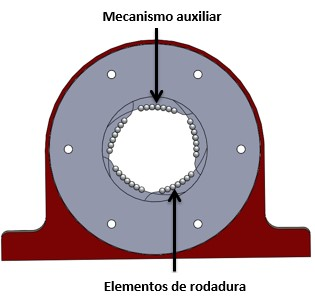
\includegraphics[scale=.90]{images/Capitulo_2/MSG}
	\caption{\textit{Diseño conceptual del dispositivo auxiliar para el módulo de seguridad.}}
	\label{fig:system:example1}
\end{figure}

\subsection{Collarín de Levitación}

Con el propósito de lograr la levitación del rotor sin importar el material del que esté fabricado, se propone el uso de un collarín de material ferromagnético que contenga al eje del rotor dentro del rodamiento. 

\begin{figure}[htb]
\centering
	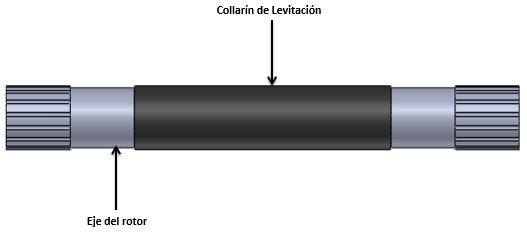
\includegraphics[scale=.90]{images/Capitulo_2/CL}
	\caption{\textit{Diseño Conceptual del collarín de levitación.}}
	\label{fig:system:example1}
\end{figure}

\subsection{Rodamiento Magnético Híbrido: Integración de los Módulos}

Aunque cada uno de los módulos es diseñado individualmente, están contemplados para funcionar de manera conjunta y ser ensamblados dentro del mismo armazón. La integración de todos los módulos nos daría como resultado el Rodamiento Magnético Híbrido. 

\begin{figure}[htb]
\centering
	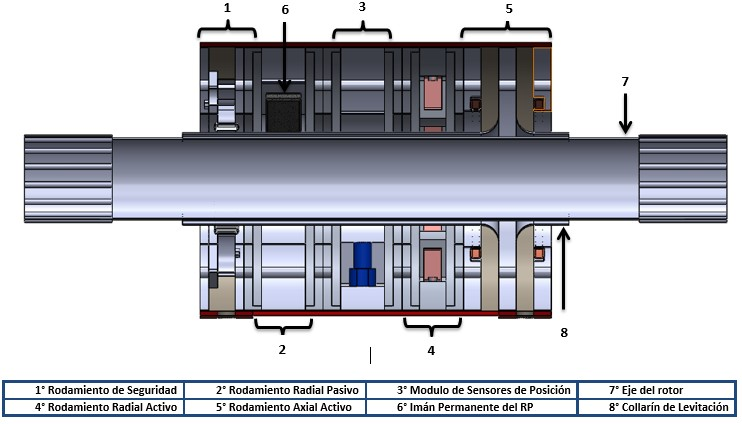
\includegraphics[width=\textwidth]{images/Capitulo_2/RMH}
	\caption{\textit{Diseño Conceptual del Rodamiento Magnético Híbrido.}}
	\label{fig:system:example1}
\end{figure}
         % INCLUDE: system
% !TEX root = ../thesis-example.tex
%
\chapter{Diseño Detallado}
\label{sec:concepts}

\cleanchapterquote{Users do not care about what is inside the box, as long as the box does what they need done.}{Jef Raskin}{about Human Computer Interfaces}

       % INCLUDE: concepts
% !TEX root = ../my-thesis.tex
%
\chapter{Conclusion}
\label{sec:conclusion}

\Blindtext[2][1]

\section{System Section 1}
\label{sec:conclusion:sec1}

\Blindtext[2][2]

\section{System Section 2}
\label{sec:conclusion:sec2}

\Blindtext[3][2]

\section{Future Work}
\label{sec:conclusion:future}

\Blindtext[2][2]
     % INCLUDE: conclusion

% --------------------------
% Back matter
% --------------------------
%
{%
\setstretch{1.1}
\renewcommand{\bibfont}{\normalfont\small}
\setlength{\biblabelsep}{0pt}
\setlength{\bibitemsep}{0.5\baselineskip plus 0.5\baselineskip}
\printbibliography[nottype=online]
\newrefcontext[labelprefix={@}]
\printbibliography[heading=subbibliography,title={Webpages},type=online]
}
\cleardoublepage

\listoffigures
\cleardoublepage

\listoftables
\cleardoublepage

\appendix\cleardoublepage
% !TEX root = ../my-thesis.tex
%
\chapter{Example Appendix}
\label{sec:appendix}

\Blindtext[1][1]

\section{Appendix Section 1}
\label{sec:appendix:sec1}

\Blindtext[1][1]

\begin{table}[h]
	\begin{tabularx}{\textwidth}{X | X | X}
		%\hline
		Alpha		& Beta			& Gamma			\\ \hline
		0			& 1				& 2				\\ \hline
		3			& 4				& 5				\\ %\hline
	\end{tabularx}
	\label{tab:table1}
	\caption{This is a caption text.}
\end{table}

\section{Appendix Section 2}
\label{sec:appendix:sec2}

\Blindtext[1][1]

\begin{table}[h]
	\begin{tabularx}{\textwidth}{X | X | X}
		%\hline
		Alpha		& Beta			& Gamma			\\ \hline
		0			& 1				& 2				\\ \hline
		3			& 4				& 5				\\ %\hline
	\end{tabularx}
	\label{tab:table2}
	\caption{This is a caption text.}
\end{table}

\Blindtext[1][2]
       % INCLUDE: appendix

\cleardoublepage
% !TEX root = ../my-thesis.tex
%
\pagestyle{empty}
\hfill
\vfill
\pdfbookmark[0]{Colophon}{Colophon}
\section*{Colophon}

This thesis was typeset with \LaTeXe.
It uses the \textit{Clean Thesis} style developed by Ricardo Langner.
The design of the \textit{Clean Thesis} style is inspired by user guide documents from Apple Inc.

Download the \textit{Clean Thesis} style at \url{http://cleanthesis.der-ric.de/}.


\cleardoublepage
% !TEX root = ../thesis-example.tex
%
%************************************************
% Declaration
%************************************************
\pdfbookmark[0]{Declaration}{Declaration}
\chapter*{Declaration}
\label{sec:declaration}
\thispagestyle{empty}

Uno nunca esta satisfecho de sus creaciones o de sus desarrollos tecnológicos hasta que un tercero vea el esfuerzo que con lleva  no físicamente sino mentalmente.  
\bigskip

\noindent\textit{\thesisUniversityCity, \thesisDate}

\smallskip

\begin{flushright}
	\begin{minipage}{5cm}
		\rule{\textwidth}{1pt}
		\centering\thesisName
	\end{minipage}
\end{flushright}

%*****************************************
%*****************************************

\clearpage

\newpage
\mbox{}

% **************************************************
% End of Document CONTENT
% **************************************************
\end{document}
